\documentclass{scrreprt}
\usepackage{listings}
\usepackage{underscore}
\usepackage{graphicx}
\usepackage[bookmarks=true]{hyperref}
\usepackage[utf8]{inputenc}
\usepackage[spanish]{babel}
\usepackage{tabularx}
\usepackage{hyperref}
\usepackage[usenames,dvipsnames]{xcolor}

\urlstyle{same}

\hypersetup{
    bookmarks=false,    % show bookmarks bar?
    pdftitle={Documento de Arquitectura de Software},    % title
    pdfauthor={Albany Armenta},                     % author
    pdfsubject={TeX and LaTeX},                        % subject of the document
    pdfkeywords={TeX, LaTeX, graphics, images}, % list of keywords
    colorlinks=true,       % false: boxed links; true: colored links
    linkcolor=blue,       % color of internal links
    citecolor=black,       % color of links to bibliography
    filecolor=black,        % color of file links
    urlcolor=purple,        % color of external links
    linktoc=page            % only page is linked
}%
\def\myversion{1.0 }
\date{}
%\title
\usepackage{hyperref}
\begin{document}

\begin{flushright}
    \rule{16cm}{5pt}\vskip1cm
    \begin{bfseries}
        \Huge{Documento de Arquitectura de Software}\\
        \vspace{1.5cm}
        \textbf{Sistema para la Recolección, Procesamiento y Clasificación a partir de Wi-Fi CSI}\\
        \vspace{1.5cm}
        \LARGE{Versión \myversion}\\
        \vspace{1.5cm}
        Elaborado por: Jesús A. Armenta-García\\
        \vspace{1.5cm}
        \today\\
    \end{bfseries}
\end{flushright}

\tableofcontents

\chapter{Introducción}

\section{Propósito}
El propósito de este documento es presentar el sistema \emph{Herramienta de Recolección, Procesamiento y Clasificación a partir de Wi-Fi CSI} y describir su arquitectura interna desde diferentes perspectivas del desarrollo de software, proporcionando una descripción detallada de las funcionalidades del sistema y las interacciones entre cada uno de los componentes internos. Esto con la finalidad de facilitar las tareas de mantenimiento o extensión de funcionalidades del sistema. 

\section{Audiencia Objetivo}
Este documento esta dirigido a desarrolladores de software, administradores de proyecto y usuarios interesados en el funcionamiento del sistema que aquí se presenta. 

\section{Alcance del Proyecto}
Para el desarrollo del sistema \emph{Herramienta de Recolección, Procesamiento y Clasificación a partir de Wi-Fi CSI} se planteó un proyecto con duración de cuatro años el cual abarcaba actividades de investigación, desarrollo, pruebas, divulgación y difusión, culminando con la difusión del sistema ante la comunidad científica para promover su utilización e impulsar el desarrollo de sistemas de monitoreo con base en señales Wi-Fi, difundiendo un caso de uso del sistema para la identificación de actividades humanas y monitoreo de frecuencia respiratoria. 

Cabe destacar que lo que se presenta en este documento corresponde al segundo de los cuatro años definidos para el proyecto, en donde las actividades se enfocaban en el proceso de desarrollo y pruebas del sistema. Por lo tanto el alcance de este documento es llegar a ofrecer, como se mencionó anteriormente, una descripción detallada de las funcionalidades del sistema y las interacciones entre los componentes internos a partir de las siguientes vistas: 
\begin{itemize}
    \item \textbf{Vista de Casos de Uso: } proporciona una idea general del sistema a nivel de requerimientos destacando los actores del sistema y las acciones que estos realizan en el mismo. El diagrama seleccionado para representar esta vista en el presente documento es el \emph{Diagrama de Casos de Uso}.
    \item \textbf{Vista Lógica: } describe la arquitectura del sistema enfocándose en la descripción de la estructura y funcionalidades del mismo. En el presente documento se utiliza un \emph{Diagrama de Componentes} para ilustrar la estructura y funcionalidades del sistema. 
    \item \textbf{Vista de Procesos: } describe los procesos del sistema y las interacciones entre ellas en el tiempo de ejecución. Para describir el sistema por medio de esta vista se hace uso de un \emph{Diagrama de Secuencia}. 
    \item \textbf{Vista de Despliegue: } describe la distribución del sistema de manera física, es decir, en donde el sistema será ejecutado y si tiene interacción con otros elementos físicos. El diagrama seleccionado para representar esta vista es el \emph{Diagrama de Despliegue}
\end{itemize}

\chapter{Descripción del Sistema}

\section{Descripción General}
El Sistema para la Recolección, Procesamiento y Clasificación a partir de Wi-Fi CSI es un sistema que tiene como propósito, en una primera iteración del sistema, la clasificación de actividades humanas utilizando modelos de aprendizaje profundo, con la particularidad que las etapas de  recolección de información, procesamiento y la clasificación con aprendizaje profundo se realiza en un dispositivo en el borde de bajo costo y consumo energético, siendo este un microcontrolador ESP32. Esto es posible aprovechando al máximo el procesador con doble núcleo con el que cuenta el microcontrolador, así como la memoria PSRAM con la que cuentan algunas placas de desarrollo de ESP32 que hacen posible almacenar un modelo de aprendizaje profundo en el dispositivo sin agotar los recursos del mismo. 

\section{Procesos del Sistema }
El sistema se divide en cinco procesos (\emph{tasks}, de acuerdo a FreeRTOS), Main Task, Wi-Fi Task, Processor Task, CSI Task y Predictor Task. 
\begin{itemize}
  \item \textbf{Main Task: } es el proceso que se inicia al encender el dispositivo. Es responsable de iniciar el proceso \emph{Wi-Fi Task} e inicializar el almacenamiento no volátil del dispositivo.
  \item \textbf{Wi-Fi Task: } proceso que se encarga de configurar los parámetros del dispositivo para que funcione como punto de acceso. Los parámetros de configuración, así como los valores que asigna este proceso se presentan en el Cuadro \ref{tab:ap_conf}. Una vez que el dispositivo es configurado como punto de acceso, este proceso se encarga de gestionar la conexión de estaciones y de reportar la CSI hacia el proceso \emph{Processor Task} de forma periódica.
  
    \begin{table}[h!]
    \caption{Valores de Configuración del Punto de Acceso}
    \begin{tabularx}{\textwidth}{|X | X |}
        \hline
        \textbf{Parámetro} & \textbf{Valor} \\
        \hline 
        SSID & CSI_Collection \\
        \hline 
        Contraseña & root1234 \\
        \hline 
        Canal Wi-Fi & 1 \\
        \hline 
        Modo de Autenticación & WPA2 PSK \\
        \hline 
    \end{tabularx}
    \label{tab:ap_conf}
    \end{table}

  \item \textbf{Processor Task: } proceso que se encarga de almacenar la CSI reportada por el proceso \emph{Wi-Fi Task} para su procesamiento. Cada que una estimación de CSI es reportada, este proceso se encarga de calcular la amplitud y fase de cada una de las subportadoras presentes en la estimación. Este proceso además cuenta con un banco de filtros de frecuencia paso-bajas, uno para cada subportadora, los cuales actúan sobre la amplitud y fase estimada para que, una vez filtrados, se almacenen en una estructura de cola que representa una ventana de muestras. Una vez que se tiene una ventana de muestras de un determinado tamaño, el proceso aplica un identificador Hampel para la sustitución de datos atípicos y, una vez aplicado, se construye una observación que será pasado al proceso \emph{Predictor Task} para la clasificación de la ventana en una de las posibles actividades humanas consideradas. 
  \item \textbf{CSI Task: } es un proceso intermedio entre el \emph{Wi-Fi Task} y el \emph{Processor Task}. Este se encarga de definir la funcionalidad que realizará el \emph{Wi-Fi Task} cada que se reciba un nuevo paquete de información y se estime la CSI. Además, se encarga de inicializar el \emph{Processor Task} una vez que la \emph{Wi-Fi Task} le notifica que se ha detectado la conexión de una estación al punto de acceso. 
  \item \textbf{Predictor Task: } proceso que se encarga de clasificar las observaciones que son enviadas por el \emph{Processor Task}. Dicha clasificación se realiza mediante un modelo de aprendizaje profundo cuya arquitectura se ilustra en la Figura \ref{fig:DL}. 
  
    \begin{figure}[h!]
        \centering
        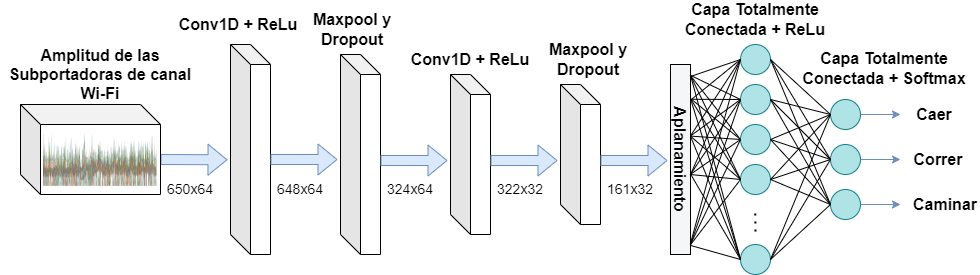
\includegraphics[scale = 0.42]{images/DL_architecture.drawio.png}
        \caption{Arquitectura del Modelo utilizado por el Predictor Task}
        \label{fig:DL}
    \end{figure}
\end{itemize}

%\section{Plataforma de Desarrollo e Implementación}
%Descripcion de ESP IDF y ESP32

\chapter{Vista de Casos de Uso}

Los actores que intervienen en el sistema, en conjunto con la descripción de cada uno de ellos se presenta en el Cuadro \ref{tab:actores}. Por otra parte, las interacciones de cada uno de ellos con el sistema se ilustran en la Figura \ref{fig:casos_uso}. 
\begin{table}[h!]
    \caption{Descripción de Actores en el Sistema}
    \begin{tabularx}{\textwidth}{|l | X |}
        \hline
        \textbf{Actor} & \textbf{Descripción} \\
        \hline 
        Administrador & El Investigador es el responsable de realizar la configuración de la etapa de recolección del sistema, teniendo que definir la direcciones MAC del dispositivo receptor y transmisor para establecer el enlace de comunicación entre ambos. \\
        \hline 
        Persona a Monitorear & Corresponde a la persona a la cual se desea monitorear por medio del sistema. Si bien este actor no ejerce de manera directa una interacción con el sistema, sus acciones son capturadas por el sistema. \\ 
        \hline 
    \end{tabularx}
    \label{tab:actores}
\end{table}

\begin{figure}[h!]
    \centering
    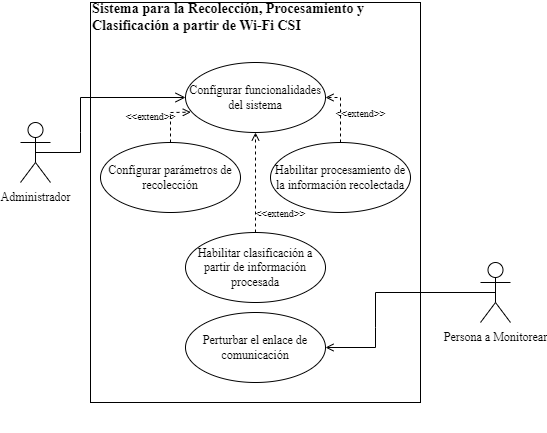
\includegraphics[scale = 0.57]{images/casos_uso.png}
    \caption{Diagrama de Casos de Uso}
    \label{fig:casos_uso}
\end{figure}

\chapter{Vista Lógica}
Para describir el sistema desde una vista lógica se utiliza un \emph{Diagrama de Componentes} el cual se muestra en la Figura \ref{fig:componentes}. En este podemos observar que los proceso del sistema también pueden ser catalogados como componentes del mismo con funcionalidades específicas e interacciones marcadas entre sí. A su vez, estos se pueden englobar en tres macro-componentes de acuerdo a la función que realizan, siendo estos \emph{Recolector, Procesador} y \emph{Clasificador}. Para el componente \emph{Processor Task} se puede observar que requiere de un conjunto de \emph{coeficientes} que son provistos por un componente \emph{Filtros}, estos corresponden a los coeficientes que son resultado de representar un filtro de frecuencia mediante una ecuación de diferencias; por lo que de ser necesario, se puede modificar el comportamiento del filtro cambiando los valores de este componente.

Por otra parte, el macro-componente \emph{Clasificador} cuenta con un componente denominado \emph{Modelo}, el cual define la arquitectura del modelo de aprendizaje profundo en forma de vector. 

\begin{figure}[h!]
    \centering
    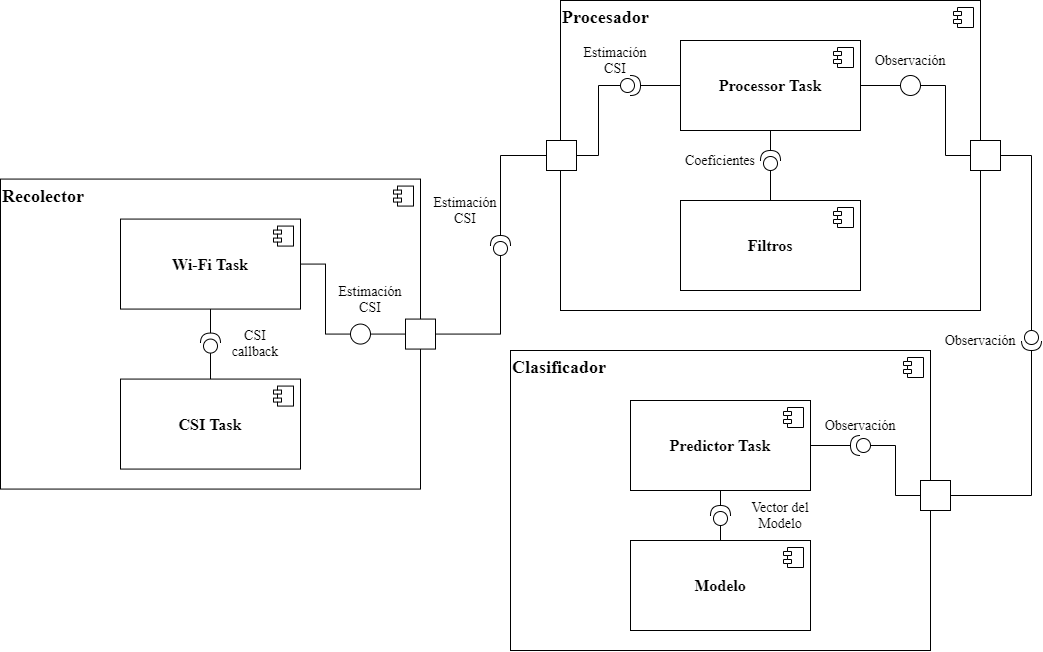
\includegraphics[scale = 0.39]{images/component.png}
    \caption{Diagrama de Componentes}
    \label{fig:componentes}
\end{figure}

\chapter{Vista de Procesos}
Las interacciones principales entre los componentes, así como la secuencia en la que ocurren, se presentan en el \emph{Diagrama de Secuencia} de la Figura \ref{fig:secuencia}. En ella se puede observar que hay un conjunto de operaciones que se realizan periódicamente en el sistema, ya que estas interacciones corresponden al proceso reportar la CSI, procesarla, construir una observación y por último clasificar con el modelo, el cual se realiza cada que se recibe una nueva estimación (una vez cada 20 milisegundos) a excepción de la clasificación que, al ser una tarea demandante de tiempo, esta se realiza únicamente una vez por segundo. 

\begin{figure}[h!]
    \centering
    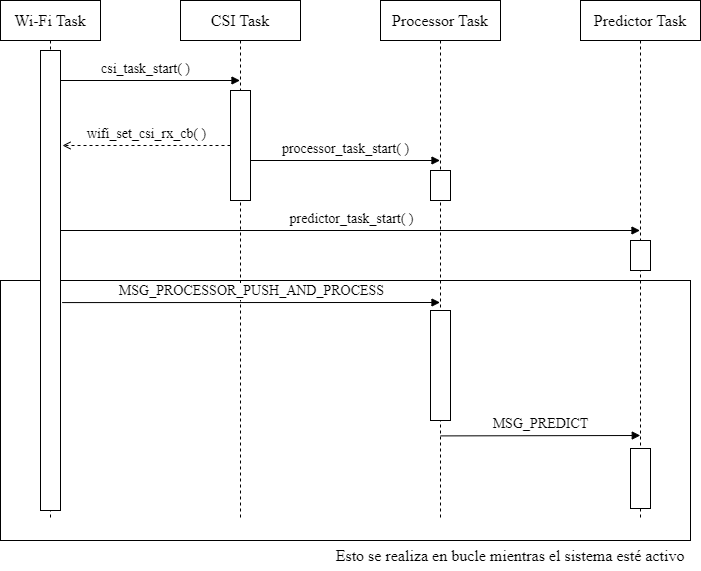
\includegraphics[scale = 0.45]{images/sequence.png}
    \caption{Diagrama de Secuencia}
    \label{fig:secuencia}
\end{figure}

\chapter{Vista de Despliegue}
El diagrama utilizado para describir el despliegue del sistema es un \emph{Diagrama de Despliegue}, el cual se muestra en la Figura \ref{fig:despliegue}. Se puede observar que para el funcionamiento del sistema se requiere de dos dispositivos ESP32, siendo el dispositivo Receptor el que cuenta con el sistema que aquí se presenta y el dispositivo Transmisor con la herramienta \emph{ESP32 CSI Web Collecting Tool}, herramienta desarrollada en una de las etapas previas de este proyecto. 

\begin{figure}[h!]
    \centering
    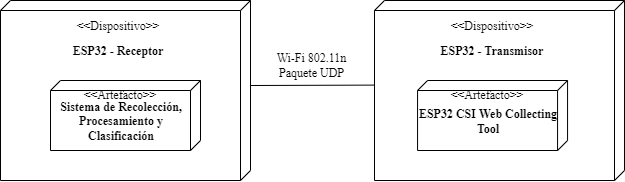
\includegraphics[scale = 0.60]{images/deployment.png}
    \caption{Diagrama de Despliegue}
    \label{fig:despliegue}
\end{figure}

\chapter{Anexos}

\section{Disponibilidad del Código}
El código que compone al sistema que se describe en este documento se encuentra en un \href{https://github.com/AlbanyArmenta0711/CSI_HAR_with_ESP32/tree/main/ESP32_Program/ESP_HAR}{repositorio de GitHub}. Sin embargo, este repositorio por el momento solo puede ser accedido por su autor. En caso de requerir acceso al mismo favor de solicitarlo.

\end{document}